%!TEX TS-program = pdflatex 
%!TEX encoding = UTF8
%!TEX spellcheck = en-US
%--------------------------
% to compile use "latexmk --pdf MotionCloudsSupplementary.tex" 
%--------------------------
\documentclass[a4paper,11pt]{article}%draft
%-------definitions-----
\newcommand{\AuthorA}{Paula~Sanz Leon}%
\newcommand{\AuthorB}{Ivo~Vanzetta}%
\newcommand{\AuthorC}{Guillaume S.~Masson} %
\newcommand{\AuthorD}{Laurent U.~Perrinet}%
\newcommand{\AddressA}{INCM, CNRS / Aix-Marseille University, France}
\newcommand{\AddressB}{Institut de Neurosciences de la Timone, CNRS / Aix-Marseille University, Marseille, France}%
\newcommand{\Website}{https://invibe.net/LaurentPerrinet}%
\newcommand{\EmailA}{Paula.Sanz@univ-amu.fr}%
\newcommand{\EmailB}{Ivo.Vanzetta@univ-amu.fr}%
\newcommand{\EmailC}{Guillaume.Masson@univ-amu.fr}%
\newcommand{\EmailD}{Laurent.Perrinet@univ-amu.fr}%
\newcommand{\Title}{%
Supplementary Videos to : \\ %
Motion Clouds: Model-based stimulus synthesis of natural-like random textures for the study of motion perception}%

%\newcommand{\Title}{%
%Supporting Information to : \\ %
%Motion Clouds: Model-based stimulus synthesis of natural-like random textures for the study of motion perception}%
%--------------------------

%%% Packages
\usepackage[utf8]{inputenc}
\usepackage[english]{babel}
%\usepackage{natbib}
\usepackage[pdftex]{graphicx} 
%\usepackage{graphics} 
%\usepackage{amssymb,amsmath,bm,amsfonts}
%\usepackage[usenames,dvipsnames]{color}
%\usepackage{float}
\usepackage[pdftex,colorlinks=true,linkcolor=black]{hyperref}
%\usepackage{multirow}
%\usepackage{subfigure}
%\usepackage{tabularx}
%\usepackage{colortbl}
%\usepackage{color}
%\usepackage{booktabs}
%\usepackage{fullpage}
%\usepackage{tikz,times}
%\usepackage{listings}
%\usepackage{fancyvrb}
%\usepackage{verbatim}
%\usepackage{alltt}
%\usepackage{watermark}
%\usepackage{fullpage}
%\usepackage{fourier}
\usepackage{nicefrac} 
%\usepackage{units}
\usepackage{authblk}
%%\usepackage[notablist,notabhead]{endfloat}
%\makeatletter
%\renewcommand{\@makecaption}[2]{%
%\vskip\abovecaptionskip
%\hbox to \hsize{\hfil #1\hfil}%
%\vskip\belowcaptionskip}
%\makeatother
%\usetikzlibrary{calc,3d}
%\usetikzlibrary{shapes,arrows}
%\captionsetup{margin=10pt,labelfont=bf}
%\usepackage[on]{auto-pst-pdf}
%\usepackage{pstricks,multido,fp,pst-coil,pst-text}
%\usepackage{pst-3dplot}

\usepackage{movie15}
%\usepackage{media9}%
%\newcommand{\includemovie}[3]{%
%\includemedia[%
%width=#1,height=#2,%
%activate=pagevisible,%
%deactivate=pageclose,%
%addresource=#3,%
%flashvars={%
%src=#3 % same path as in addresource!
%&autoPlay=true % default: false; if =true, automatically starts playback after activation (see option �activation)�
%&loop=true % if loop=true, media is played in a loop
%&controlBarAutoHideTimeout=0 %  time span before auto-hide
%}%
%]{}{StrobeMediaPlayback.swf}%
%}%
%%% Declarations and definitions
%
% %new float to avoid putting the tables at the end when using endfloat package
%\floatstyle{plain}
%\newfloat{mytable}{thp}{lop}
%\floatname{mytable}{Table}
%

\DeclareGraphicsExtensions{.jpg,.pdf,.png,.tiff}%.bmp,.mps,
\graphicspath{{../results/},{results/}}
\hypersetup{
 unicode=false, % non-Latin characters in Acrobat�??s bookmarks
	pdftitle={Supplementary Material: Motion Clouds},%
	pdfauthor={\AuthorA < \EmailA > \AddressB - \AuthorB < \EmailB > - \AuthorC < \EmailC > - \AuthorD < \EmailD > },% \Website},% 
	%pdfkeywords={\Keywords},%
	%pdfsubject={\Acknowledgments}%
 pdfcreator={LaTeX}, 	% creator of the document
 pdfproducer={LUP,PSL}, 			% producer of the document
 colorlinks=true, % false: boxed links; true: colored links
 linkcolor = black, 	% color of internal links
 citecolor = black, 	% color of links to bibliography
 filecolor = black, 			 % color of file links
 urlcolor = black 		 % color of external links
}
\title{\Title}%
\date{}%
\author[1,2]{\AuthorA \thanks{\EmailA}}
\author[1,2]{\AuthorB \thanks{\EmailB}}
\author[1,2]{\AuthorC \thanks{\EmailC}}
\author[1,2]{\AuthorD \thanks{Corresponding Author, \EmailD }}%, \Website}}
\affil[1]{\AddressA}
\affil[2]{\AddressB}

%\newcommand{\skipme}[1]{} % #1
%
%\newcommand{\hgid}{null}
%\def\baselinestretch{1.3}%
%\usepackage{lineno}
%\linenumbers
%\setpagewiselinenumbers
%\newcommand{\HRule}{\rule{\linewidth}{0.5mm}}

\begin{document}
\maketitle
%\vspace{-1cm}
%
%%%%%%%%%%%%%%%%%%%% Include files %%%%%%%%%%%%%%%%%%%%%%%%%%%%%%
%
%
%
%We have defined Motion Clouds (MCs) as Random Phase Textures (RPTs)  with 1) a constant, whole-field translational motion $\vec{V}$ and 2) an optimal spread of spectral energy in the Fourier domain. Moreover, natural-like RPTs are defined with a specific envelope $\mathcal{E}_{\bar{\beta}}$ as: 
%
%\begin{equation}
%\mathbf{I}(x, y, t) = \mathcal{F}^{-1}\left\{\mathcal{E}_{\bar{\beta}}(f_x,f_y,f_t) \cdot \exp^{i\phi(f_x,f_y,f_t)}\right\}
%\label{eq:fourier_image}
%\end{equation}
%
%
%The implementation presented herein is based on a simplified parametrization of the envelope of the amplitude spectrum. Indeed, given that speed, radial frequency and orientation spread are independent, we define separate definitions of MCs based on these components. Thus, we choose this type of parametrization for our generative model:  such a 3D Gaussian envelope would be fully characterized by 3 parameters for the mean values and 6 parameters for the symmetric covariance matrix. Moreover, we have defined the parameters of 2D motion (speed and orientation) and the average spatial frequency of the texture (radial and orientation) by using their Fourier equivalent in spherical coordinates: respectively a frequency radius - the radial component-, the speed plane orientation - the polar component -, and the tilt of this plane - the azimuthal component. As a consequence, these envelopes are defined in  uncorrelated coordinates, this is to say that and one can modify the parameters of each envelope  independently. It shall be noticed that actual values of each of these parameters can be set based on known properties of the biological system to be investigated, for each level of observation.
%
%
%\paragraph{Speed Envelope}
%
%The orientation and tilt of the plane are determined by the direction and speed of motion, respectively. For larger $V=\| \vec{V} \|=\sqrt{V_x^2+V_y^2}$, the tilt  becomes greater. To model variability of speed in a motion cloud, we will assume that motion  varies slightly in both axis of speed (direction and amplitude). The envelope is given by:
%\begin{equation}
%\mathcal{V}_{(V_x, V_y, B_{V})}(f_{x}, f_{y}, f_{t})=\exp\left(-\dfrac{1}{2}\left( \dfrac{ f_x\cdot V_x + f_y\cdot V_y + f_t }{B_{V} \cdot f_r} \right)^{2} \right)
%\label{eq:envelope_speed_plane}
%\end{equation}
%where  $ f_r = \sqrt{f_x^2 + f_y^2 + f_t^2} $ is the radial frequency. Some examples are shown in figure~\ref{fig:radial_speed_plane}. 
%
%%% REMOVED (the outline of the proof and the proof should be as supplementary material or maybe for another journal, right?): 
%We outline here a proof for Equation~\ref{eq:envelope_speed_plane}. The speed envelope is defined by slow perturbations followed by a tilt of the speed plane normal to $\vec{V}$. The infinitesimal volume corresponding to the speed range $[V, V+dV)$ is the volume in between the two planes whose tilts are defined by respectively $V$ and $V+dV$. Looking at the orientation range, $[\theta, \theta+d\theta)$ defines a  volume which corresponds to a known probability $p(V)dVd\theta$ since perturbations are independent in all directions.  The density within this volume is uniform but the density mass will decrease with respect to $f_r$ as infinitesimal volumes gets linearly "thicker" with greater frequencies. Variability of speed $V$ is then parametrized by a probability density function as a Gaussian function of mean $V$ and bandwidth $B_{V}$. Such infinitesimal volumes form a partition of the Fourier space when speeds $V$ vary over the real axis range and orientation describes $[0, 2\pi)$. We thus define the speed envelope as the probability mass function in Equation~\ref{eq:envelope_speed_plane}. %

%
\begin{figure}%[h!]
\begin{center}
\begin{tabular}{cc} 
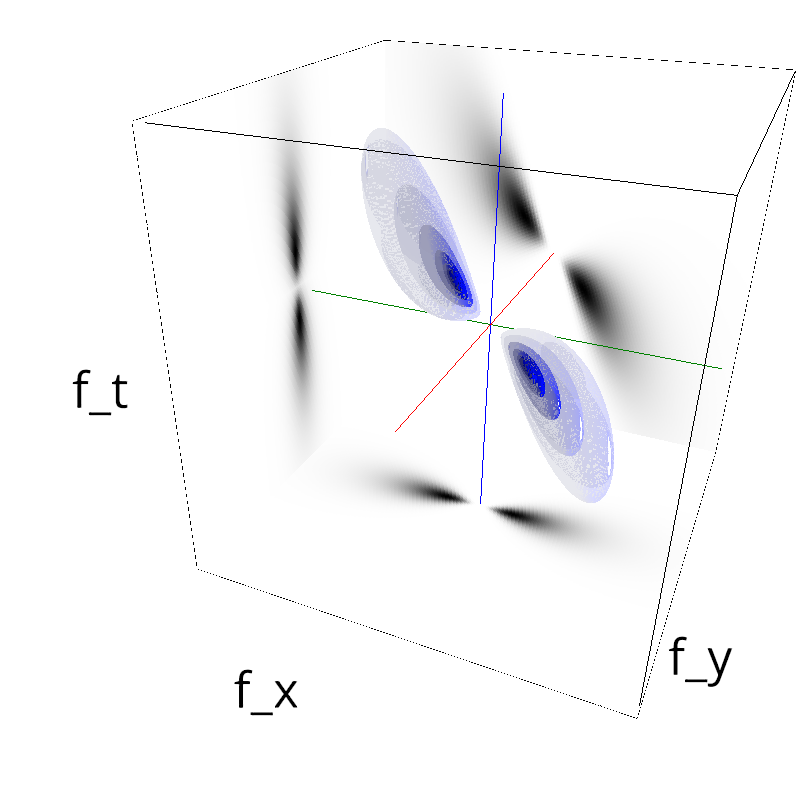
\includegraphics[width=.5\textwidth]{../results/speed-V_X-1_0.png}&
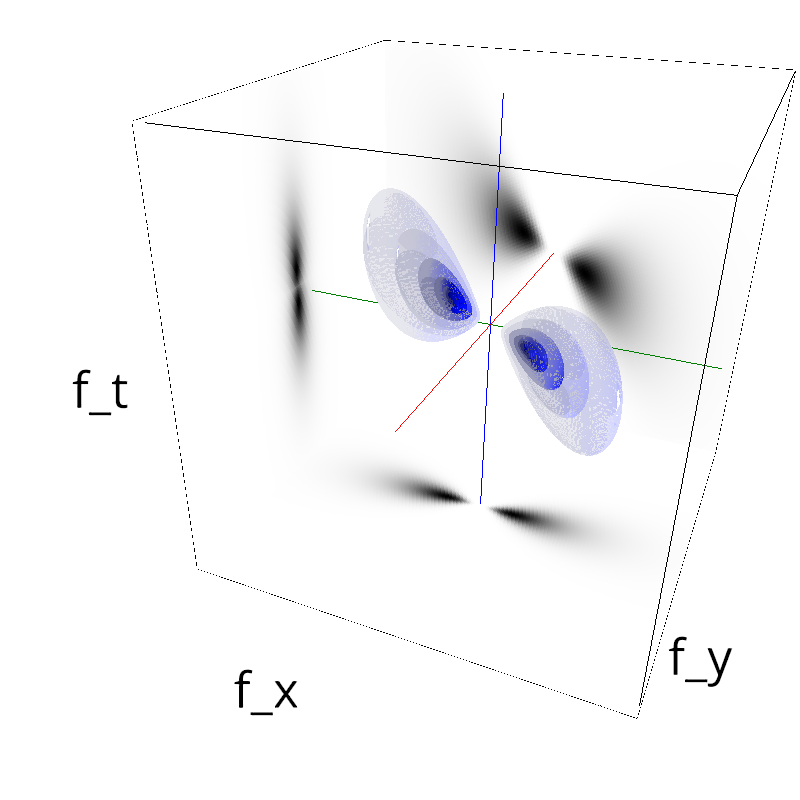
\includegraphics[width=.5\textwidth]{../results/speed-V_X-0_5.png}\\
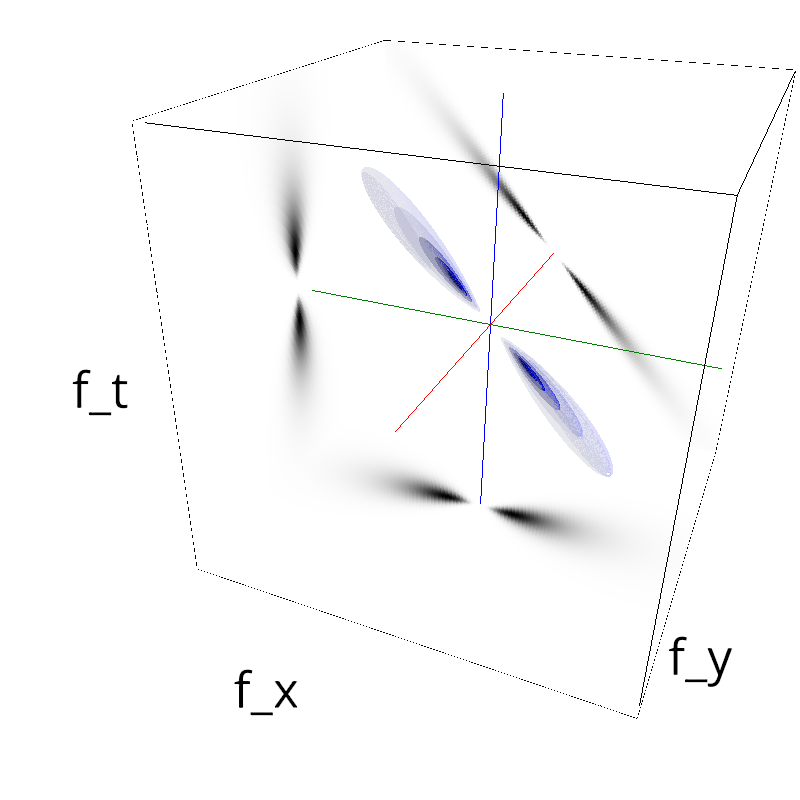
\includegraphics[width=.5\textwidth]{../results/speed-B_V-0_1.png}&%
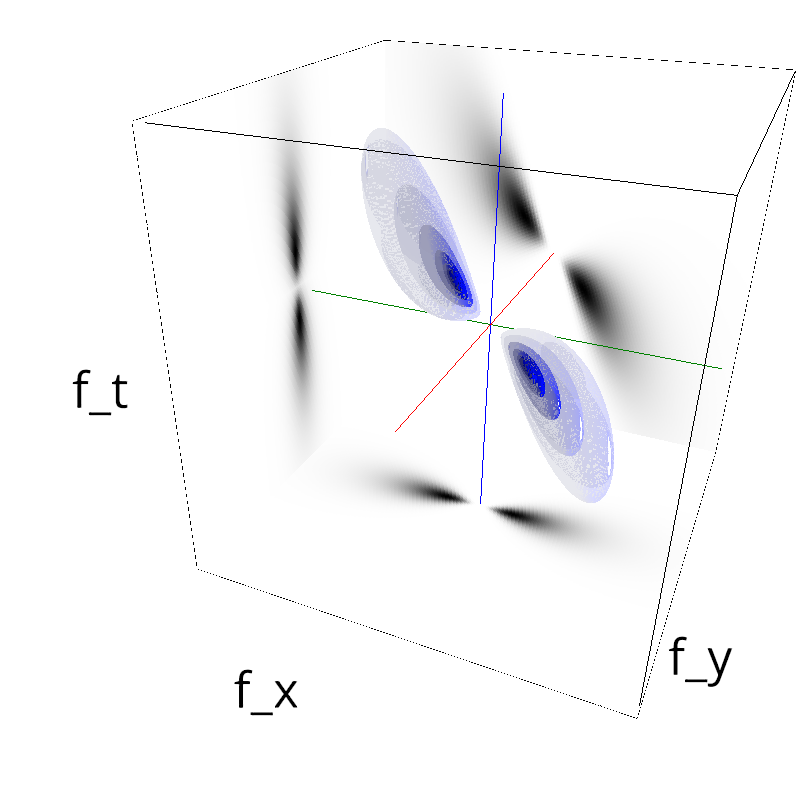
\includegraphics[width=.5\textwidth]{../results/speed-B_V-0_5.png}
\end{tabular}
\end{center}
	    \caption{We show how speed is represented in the Fourier domain. The plane where most amplitude spectrum is concentrated and that goes through the origin is the speed plane. (Upper row):  we present stimuli moving horizontally at two different speeds, $V_X=1.0$ (left) and $V_X=0.5$ (right). In this case, imagine that if we project the speed plane into the $f_x-f_t$ plane, the tilt $\nu$ of the line of intersection between both planes (and thus the tilt of the speed plane) changes as a function of $V_X$. In this way, observe that speed can be defined as $V_X=\tan(\nu)=\nicefrac{ft}{fx}$. (Lower row): the variability of speed $V$ is modeled as a Gaussian of bandwidth $B_V$ in the frequency domain. Here, we illustrate two bandwidth values $B_V=0.1$ (left) and $B_V=0.5$ (right). The plane thickness also increases as a function of frequency.}
	    \label{fig:radial_speed_plane}
\end{figure}
\begin{figure}%[h!]
\begin{center}
\begin{tabular}{cc} 
\includemovie{.5\linewidth}{.5\linewidth}{../results/speed-V_X-1_0.mp4}&
\includemovie{.5\linewidth}{.5\linewidth}{../results/speed-V_X-0_5.mp4}\\
\includemovie{.5\textwidth}{.5\textwidth}{../results/speed-B_V-0_1.mp4}&%
\includemovie{.5\textwidth}{.5\textwidth}{../results/speed-B_V-0_5.mp4}
\end{tabular}
\end{center}
	    \caption{Corresponding movies of the changes in the speed plane presented in Figure~\ref{fig:radial_speed_plane}.}
	    \label{fig:radial_speed_plane_mp4}
\end{figure}

%
%\paragraph{Radial frequency envelope}
%
%The second characteristic of a Motion  Cloud is its radial envelope. This will be defined as the one-dimensional distribution of radial frequency in spherical coordinates of the Fourier domain. We thus  build a spatial frequency band Gaussian filter that depends on the logarithm of the spatial radial frequency. We define $sf_0$ as the mean radial frequency and $B_{sf}$ is the filter's bandwidth (see figure~\ref{fig:radial_sf_0}). 
\begin{figure} %[h!]
\begin{center}
\begin{tabular}{ccc} 
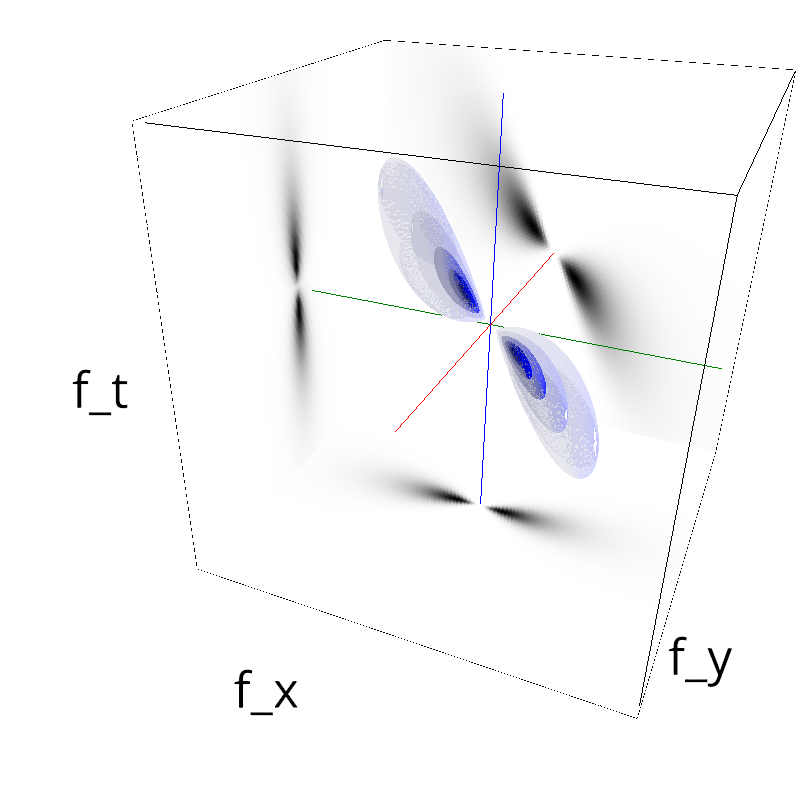
\includegraphics[width=.31\textwidth]{radial-sf_0-0_1.png}&%
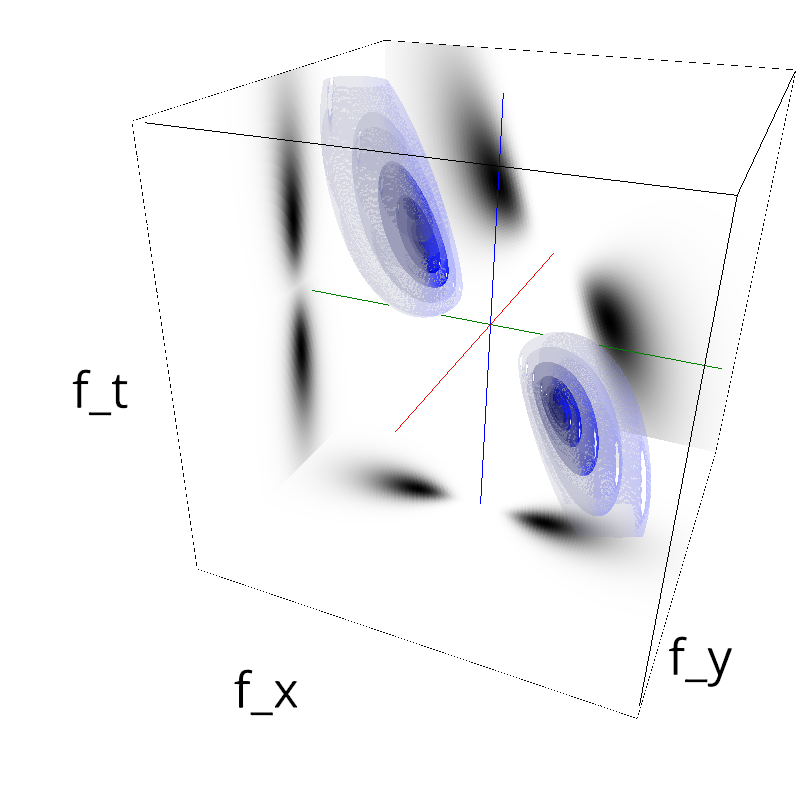
\includegraphics[width=.31\textwidth]{radial-sf_0-0_2.png}&% standard MC
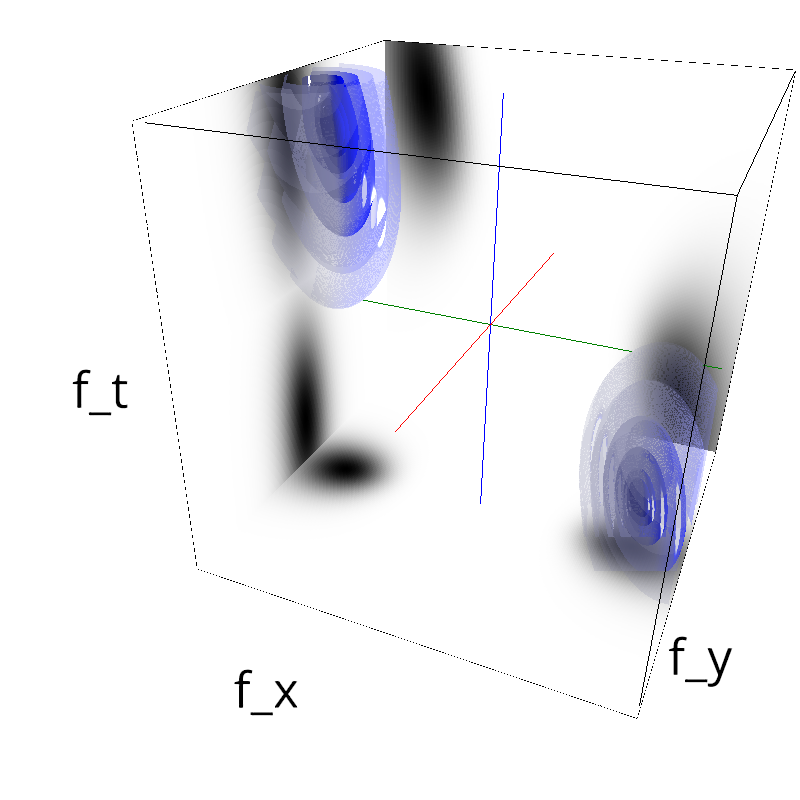
\includegraphics[width=.31\textwidth]{radial-sf_0-0_4.png}%
\\%
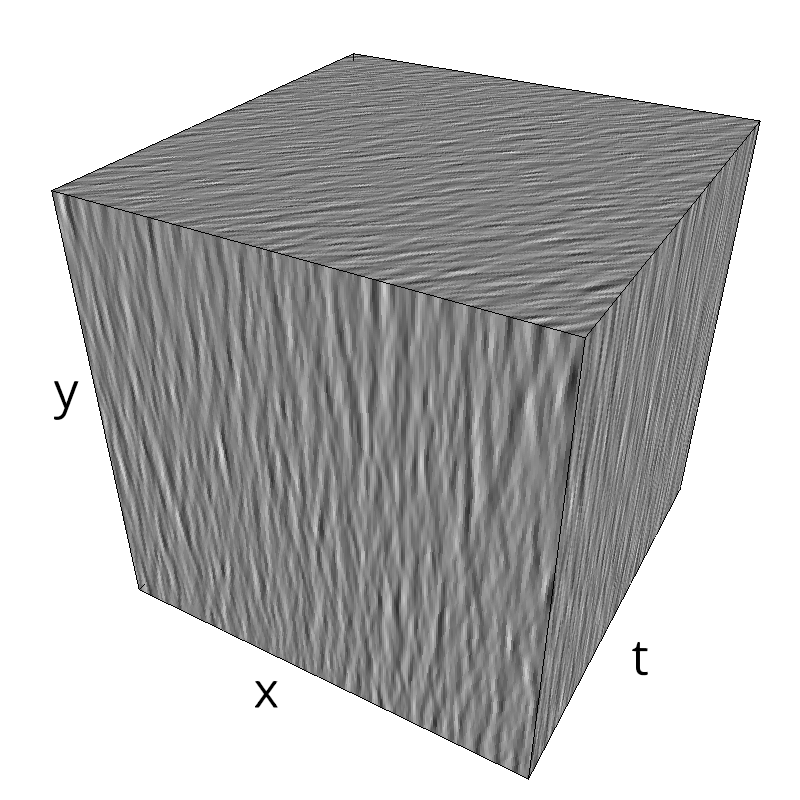
\includegraphics[width=.31\textwidth]{radial-sf_0-0_1_cube.png}&%
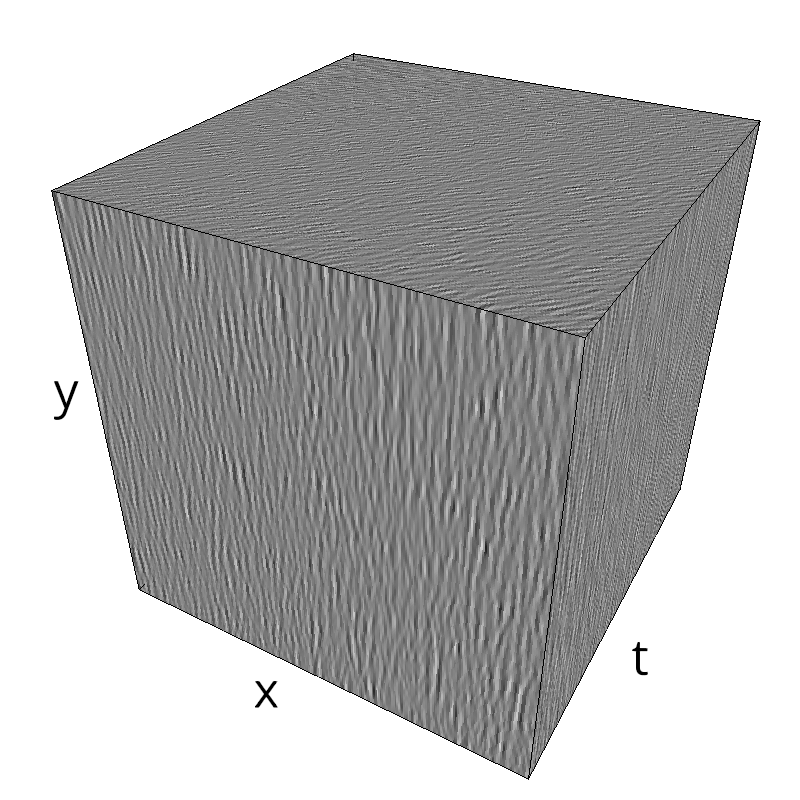
\includegraphics[width=.31\textwidth]{radial-sf_0-0_2_cube.png}&%
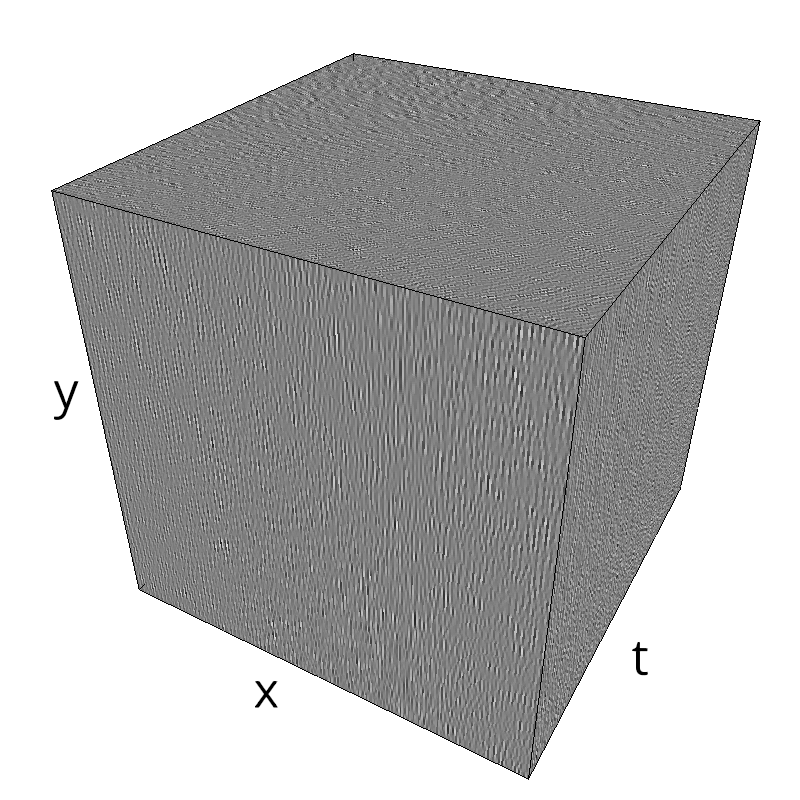
\includegraphics[width=.31\textwidth]{radial-sf_0-0_4_cube.png}%
\\%
\includemovie{.31\textwidth}{.31\textwidth}{../results/radial-sf_0-0_1.mp4}&%
\includemovie{.31\textwidth}{.31\textwidth}{../results/radial-sf_0-0_2.mp4}&% standard MC
\includemovie{.31\textwidth}{.31\textwidth}{../results/radial-sf_0-0_4.mp4}%
\end{tabular}
\end{center}
	    \caption{Spectra and stimulus cubes displaying the effect of different $sf_0$ values for a given selection of the speed plane. From right to left: increasing values of central spatial frequency. Not only the peak amplitude moves away from the origin but also the envelope spread widens from the definition of frequency bandwidth. From left to right, $sf_0$ values are $0.1$, $0.2$ and $0.4$, while $B_sf=0.2$. This stimuli are therefore simply scaled by the $sf_0$ parameter.} % TODO: check that the parameters are in sync with generate_figures.py
	    \label{fig:radial_sf_0}
\end{figure}

%
%\paragraph{Orientation Envelope}
%The third property of a Motion Cloud is its orientation envelope. Oriented structures in space-time yield oriented structures in the Fourier domain as illustrated in Fig.~\ref{fig:grating_theta}. Note that this envelope is independent upon both speed and radial frequency. Moreover, if we change in Fig. ~\ref{fig:grating_B_theta} we illustrate the effect of the parameter $B_{\theta}$. If it has a small value, a highly coherent orientation pattern is generated and it asymptotically tends to a grating-like texture. On the contrary, with a very large bandwidth, the global envelope is isotropic and contains all orientations.

\begin{figure} 
\begin{center}
\begin{tabular}{ccc} 
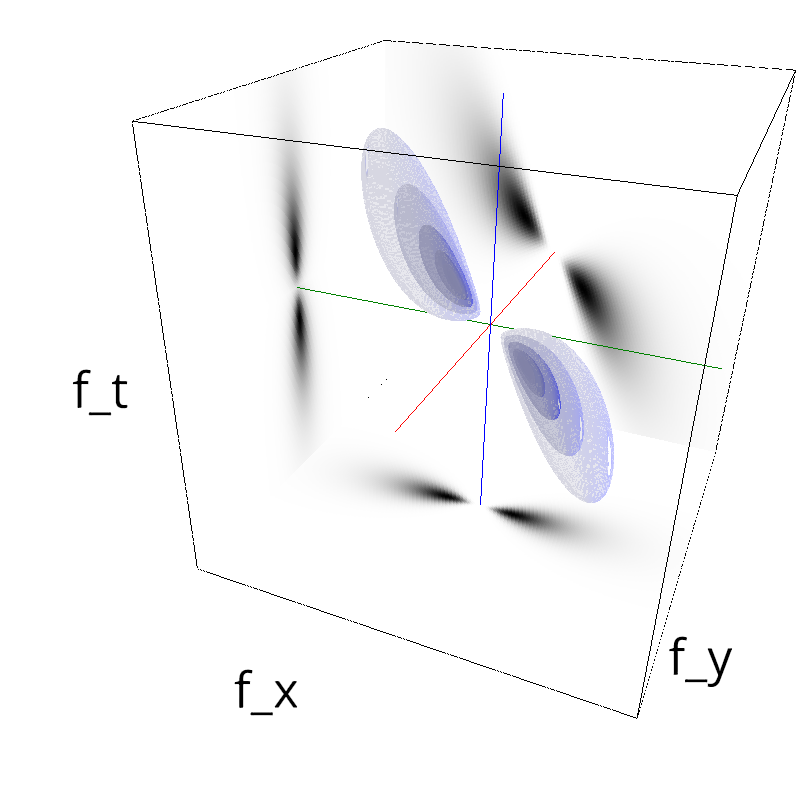
\includegraphics[width=.31\textwidth]{grating.png}&%
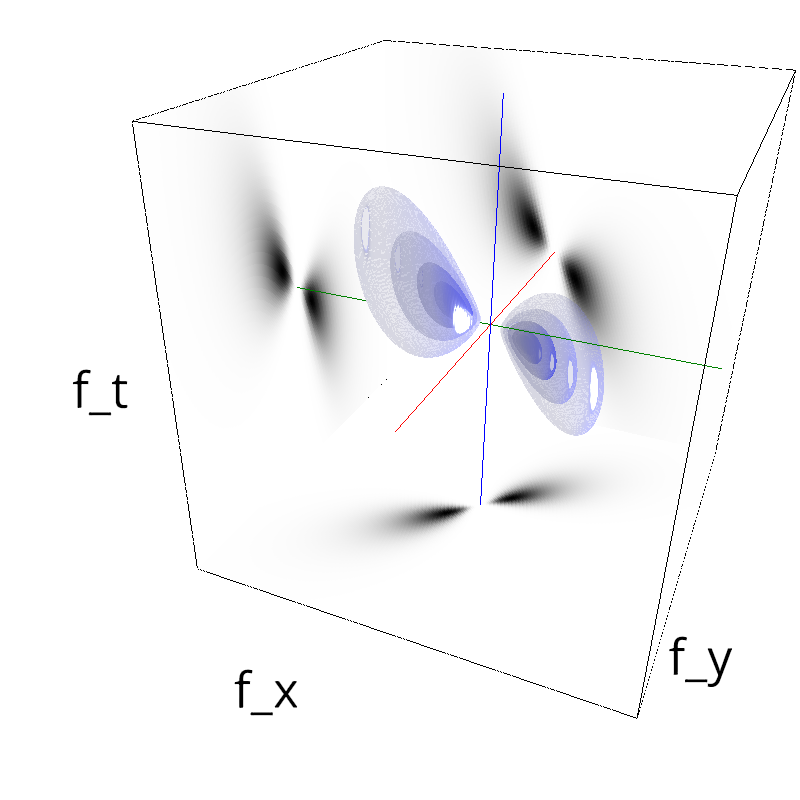
\includegraphics[width=.31\textwidth]{grating-theta-pi-over-4.png}&%
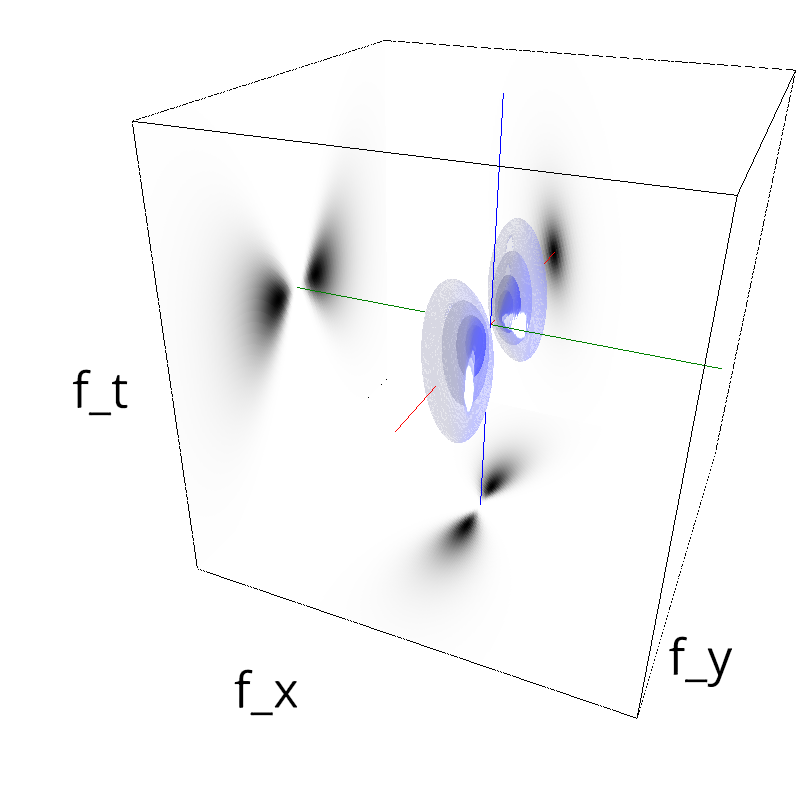
\includegraphics[width=.31\textwidth]{grating-theta-pi-over-2.png}%
\\%
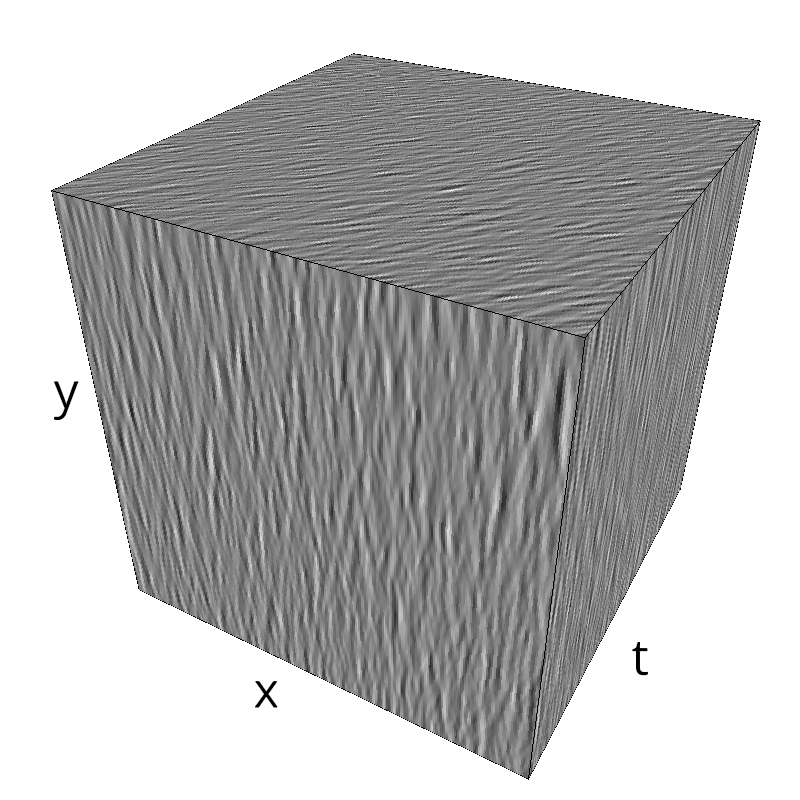
\includegraphics[width=.31\textwidth]{grating_cube.png}&%
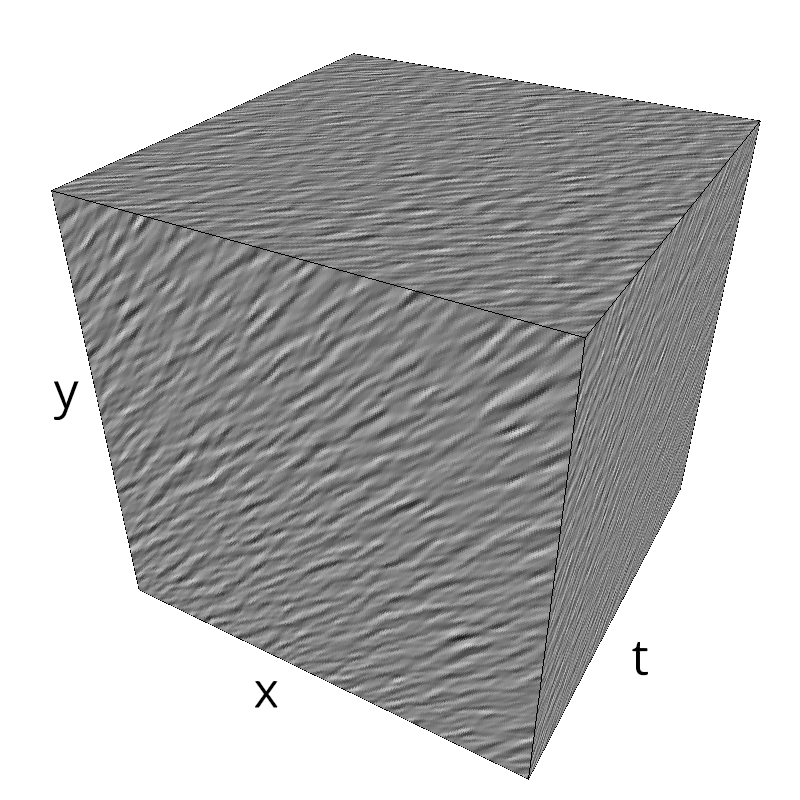
\includegraphics[width=.31\textwidth]{grating-theta-pi-over-4_cube.png}&%
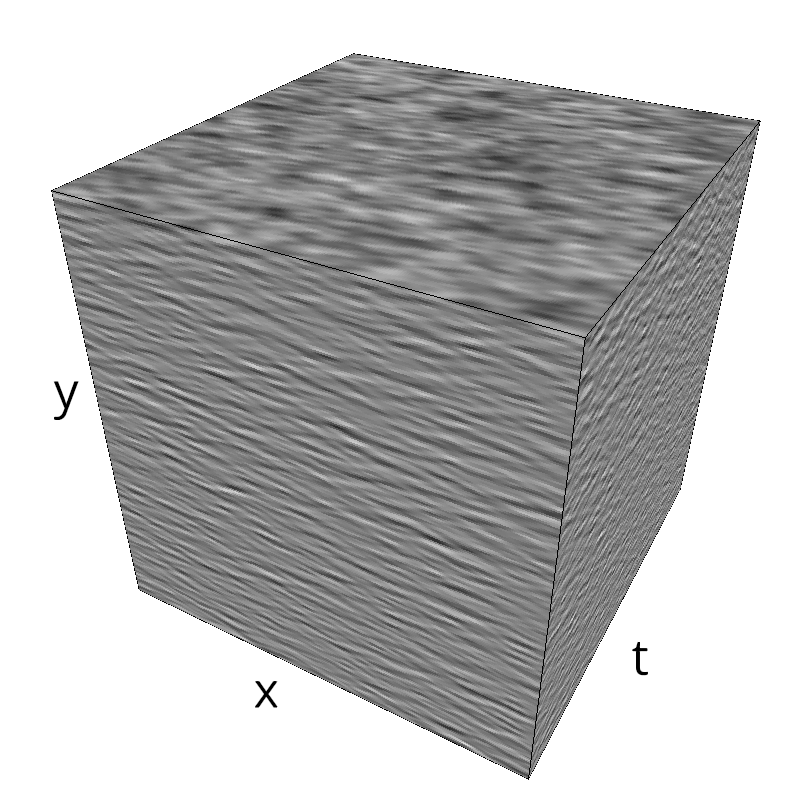
\includegraphics[width=.31\textwidth]{grating-theta-pi-over-2_cube.png}%
\\%
\includemovie{.31\textwidth}{.31\textwidth}{../results/grating-theta-pi-over-8.mp4}&%
\includemovie{.31\textwidth}{.31\textwidth}{../results/grating-theta-pi-over-4.mp4}&% standard MC
\includemovie{.31\textwidth}{.31\textwidth}{../results/grating-theta-pi-over-2.mp4}%
\end{tabular}
\end{center}
	    \caption{In this figure we illustrate the effect of parameter $\theta$: the kernel preferred orientation. We show three differently oriented narrow-orientation-bandwidth Motion Clouds (respectively $0$, $\pi/4$ and $\pi/2$ from left to right), both in the Fourier (upper row) and spatiotemporal (lower row) domains. Changes in the preferred orientation can be seen in the $x-y$ plane that corresponds to the spatial image domain, whereas in the frequency domain orientation is encoded by the relative position of the blobs with respect to the origin. Note that for $\theta=\pi/2$, the orientation is parallel to the direction, a situation that may lead to ambiguities in detecting motion similarly to the aperture problem.}
	    \label{fig:grating_theta}
\end{figure}
%
\begin{figure} %[h!]
\begin{center}
\begin{tabular}{ccc} 
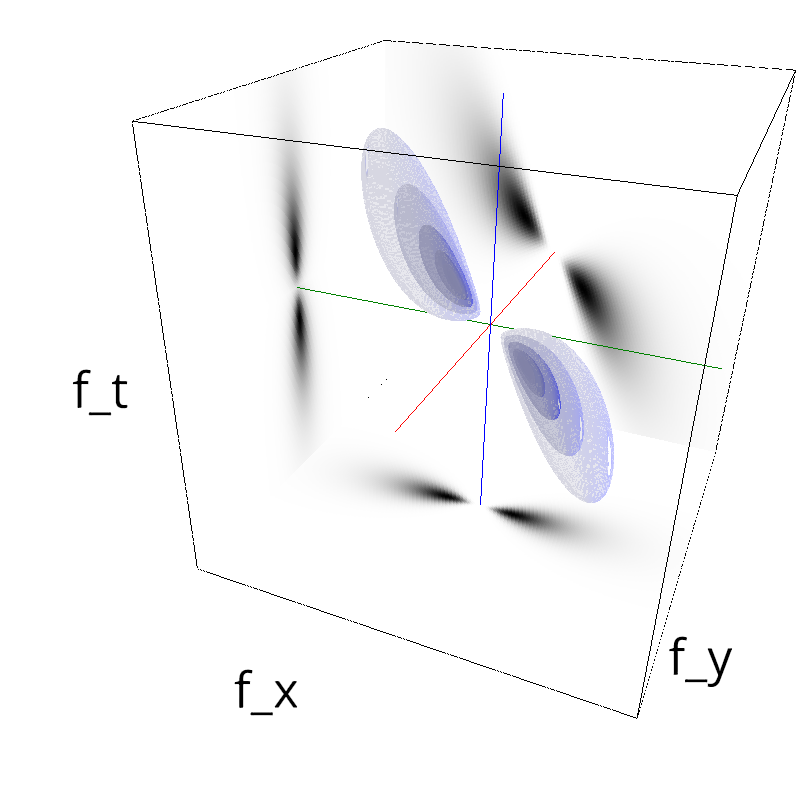
\includegraphics[width=.31\textwidth]{grating.png}&%
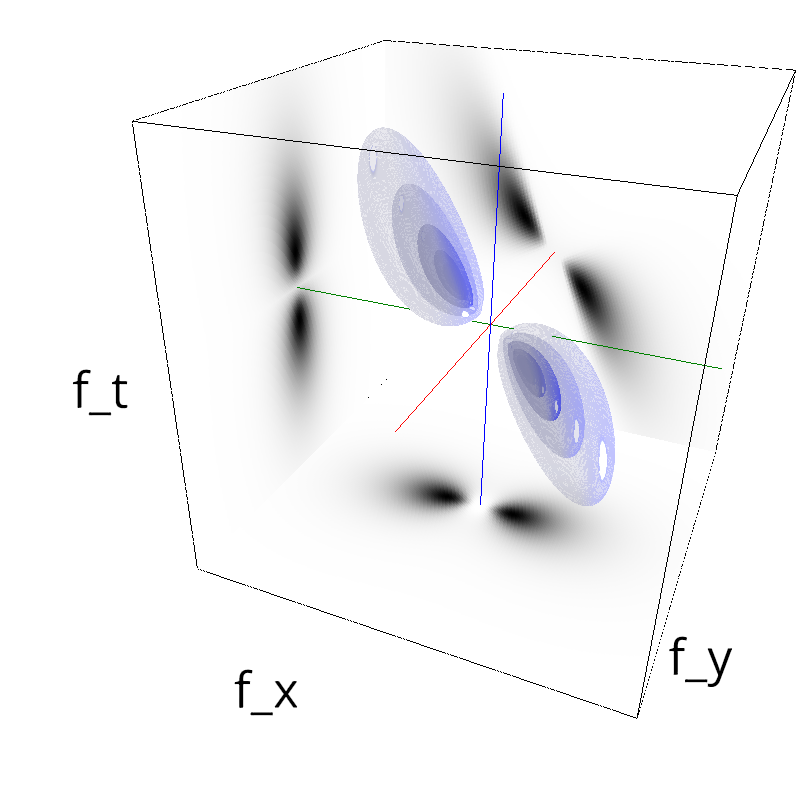
\includegraphics[width=.31\textwidth]{grating-B_theta-pi-over-8-V_X-1_0.png}&%
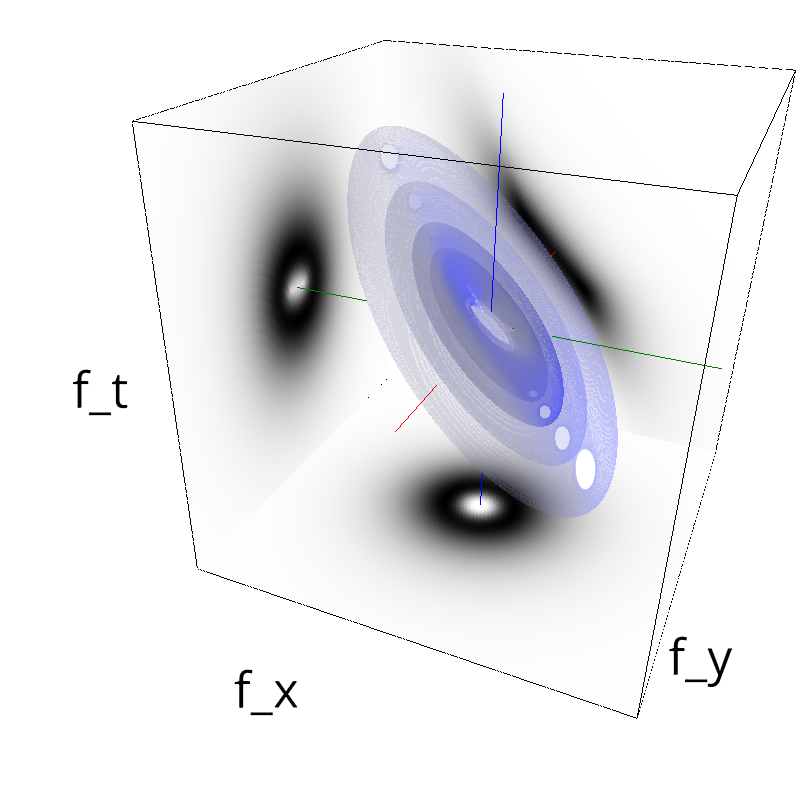
\includegraphics[width=.31\textwidth]{grating-B_theta-pi-over-1-V_X-1_0.png}%
\\
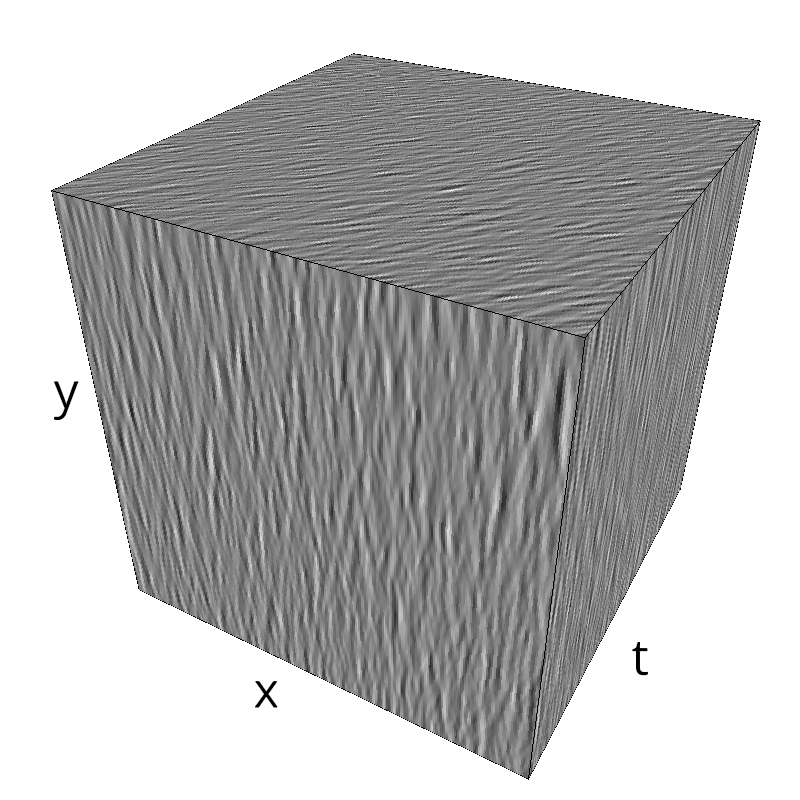
\includegraphics[width=.31\textwidth]{grating_cube.png}&%
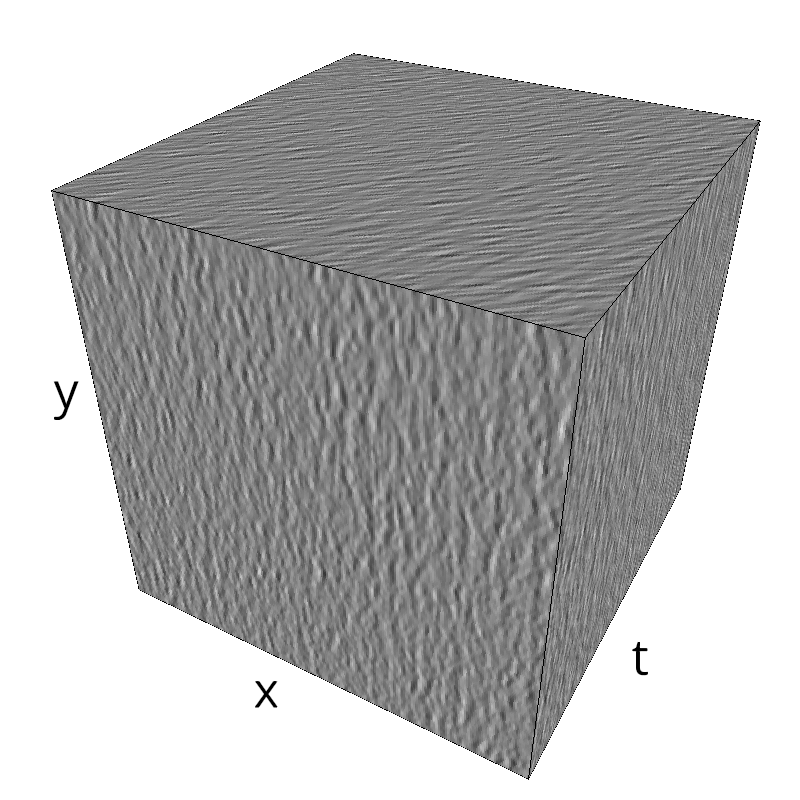
\includegraphics[width=.31\textwidth]{grating-B_theta-pi-over-8-V_X-1_0_cube.png}&%
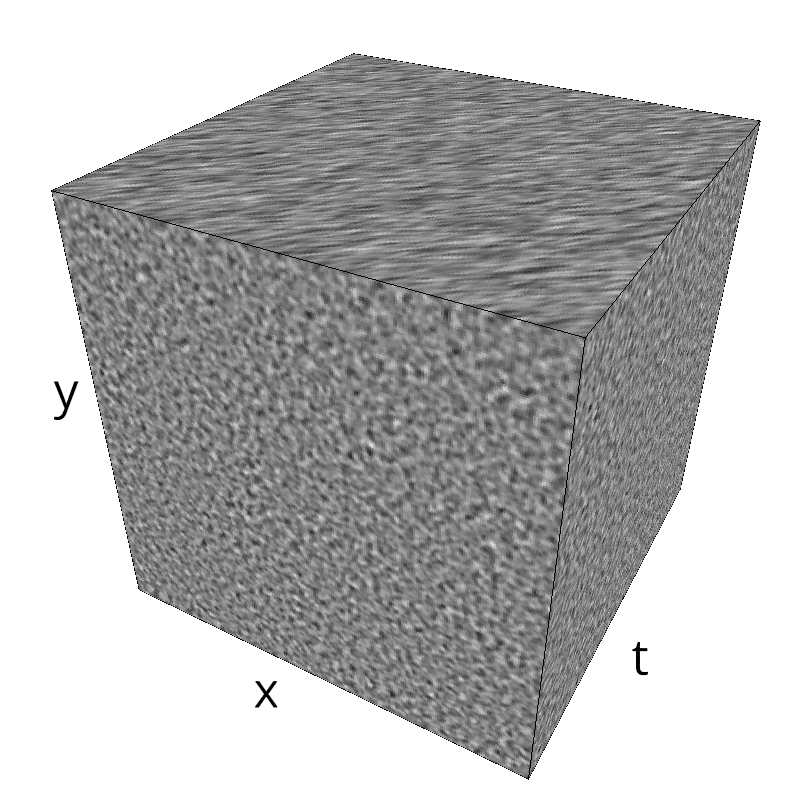
\includegraphics[width=.31\textwidth]{grating-B_theta-pi-over-1-V_X-1_0_cube.png}%
\\%
\includemovie{.31\textwidth}{.31\textwidth}{../results/grating-B_theta-pi-over-13-V_X-1_0.mp4}&% TODO is that grating.mpg?
\includemovie{.31\textwidth}{.31\textwidth}{../results/grating-B_theta-pi-over-8-V_X-1_0.mp4}&% standard MC
\includemovie{.31\textwidth}{.31\textwidth}{../results/grating-B_theta-pi-over-1-V_X-1_0.mp4}%
\end{tabular}
\end{center}
	    \caption{Motion Cloud stimuli with increasing $B_{\theta}$ from left to right. All stimuli have the same spatial frequency. On the left: a narrow orientation bandwidth stimulus ($B_\theta = \pi/13$). Its Fourier spectrum is two symmetric small aerofoil-shaped envelopes around the origin, concentrated in $sf_{0}$ and $\theta$. Middle: an intermediate bandwidth $B_\theta = \pi/8$. On the right: A cloud stimulus has a large $B_{\theta}$ and oriented edges are lost ($B_\theta = \pi$). Its spectrum is disk-shaped as in Figure~\ref{fig:radial_sf_0}-right.}
	    \label{fig:grating_B_theta}
\end{figure}

%\paragraph{Color Envelope}
% It has been shown that the average power spectrum of natural scene follows a power law:%~\citep{Field87}:
%\begin{equation}
%\mathcal{C}_{\alpha}(f_{x}, f_{y}, f_{t}) = \dfrac{1}{f_{\mathit{R}}^\alpha}
%\label{eq:powerlaw}
%\end{equation}
%where $\alpha$  is usually set within the range  $0 < \alpha < 2$. In analogy to the color terminology used to characterize noise patterns, we call this function \textit{color envelope}. The simplest stimulus that can be built with our model is filtered spatial noise as a function of the power factor $\alpha$ (see Fig. \ref{fig:pink_noise}).
%
%\begin{figure} %[h!]
%\begin{center}
%\begin{tabular}{ccc}
%	\includegraphics[width=.31\textwidth]{color-alpha-0_0_cube.png} & 
%	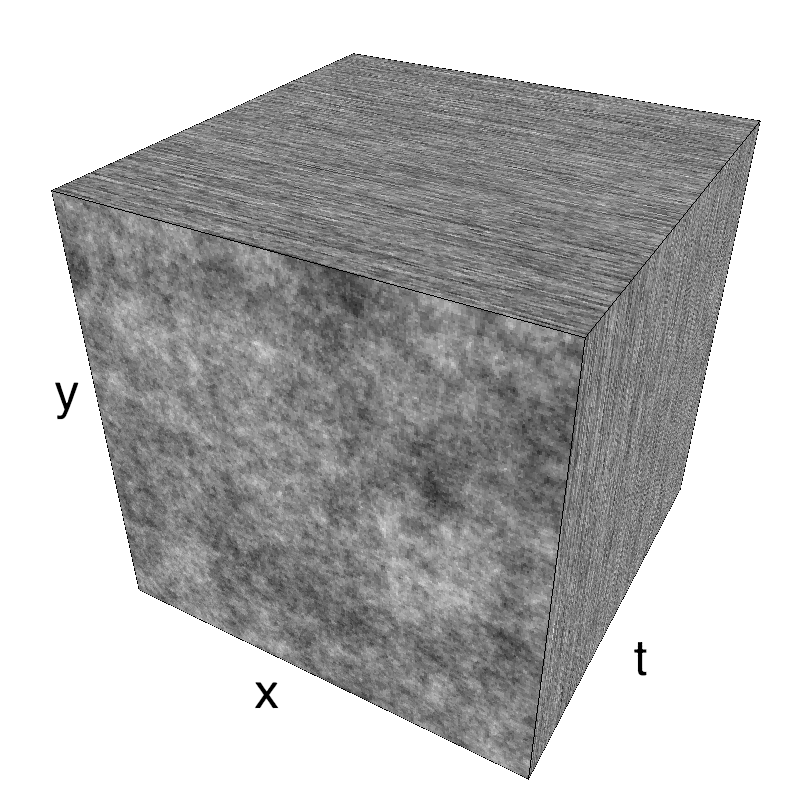
\includegraphics[width=.31\textwidth]{color-alpha-1_0_cube.png} &
%	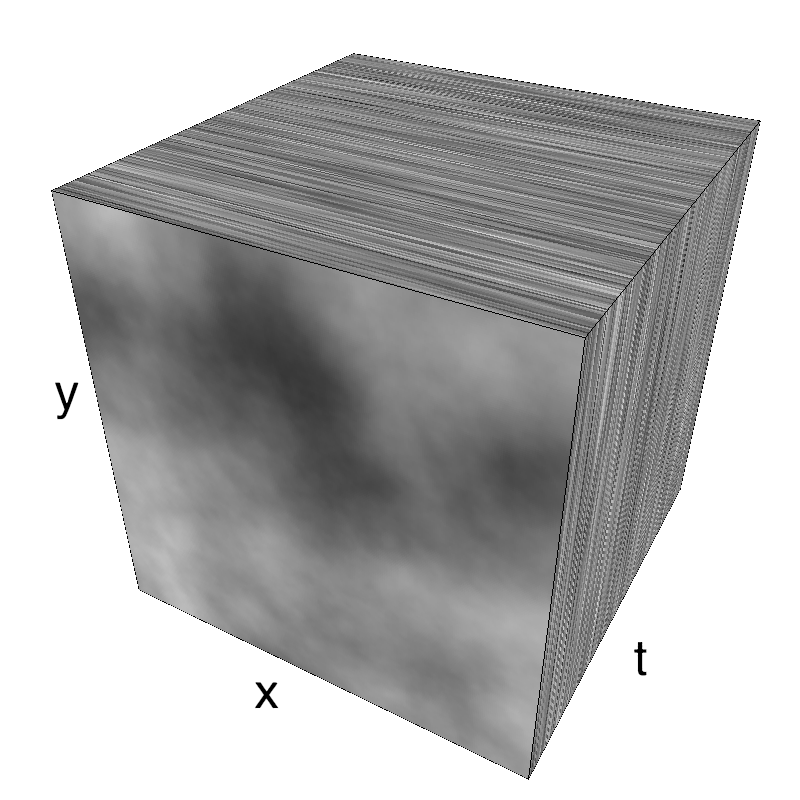
\includegraphics[width=.31\textwidth]{color-alpha-2_0_cube.png}
%%\\%
%%\includemovie{.31\textwidth}{.31\textwidth}{color-alpha-0_0.mp4}&%
%%\includemovie{.31\textwidth}{.31\textwidth}{color-alpha-1_0.mp4}&% standard MC
%%\includemovie{.31\textwidth}{.31\textwidth}{color-alpha-2_0.mp4}%
%\end{tabular}
%\end{center}
%\caption{From left to right: Image cubes of white ($\alpha=0$), pink ($\alpha=1$) and red ($\alpha=2$) spatial noise. Pink corresponds to the best fit to the average spectrum of  natural scenes and is chosen here to modulate the average spectrum of Motion Clouds.}
%	    \label{fig:pink_noise}
%\end{figure}

\begin{figure} %[h!]
\begin{center}
\begin{tabular}{ccc} 
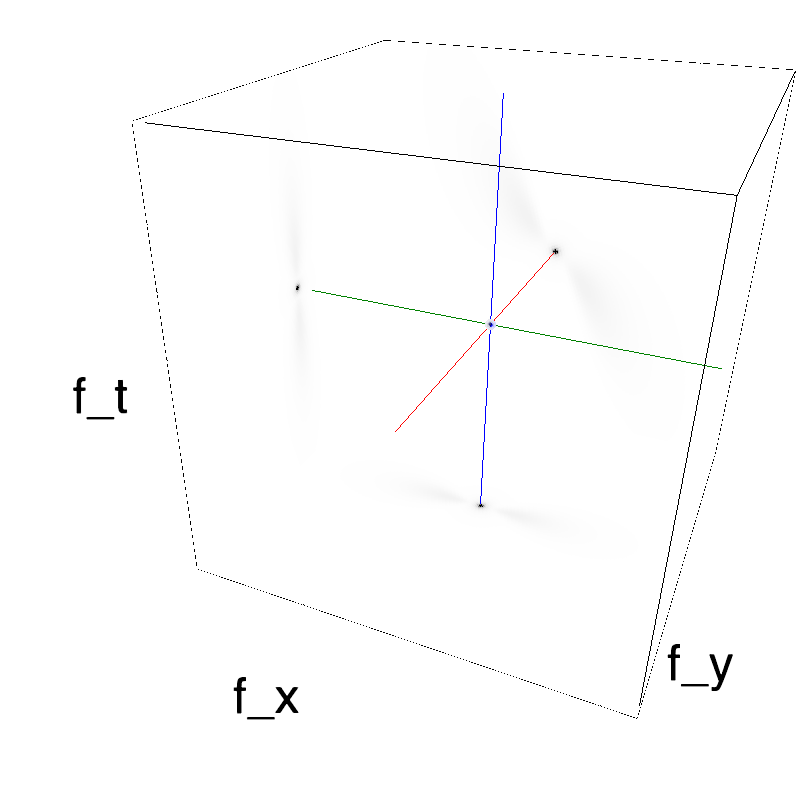
\includegraphics[width=.31\textwidth]{grating-noise.png}&%
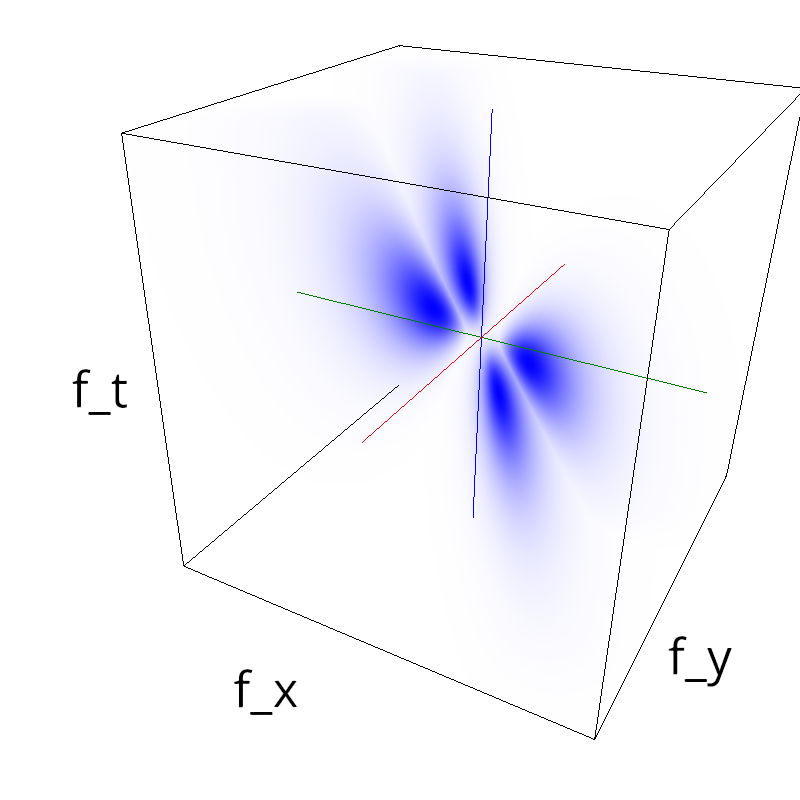
\includegraphics[width=.31\textwidth]{plaid.png}&%
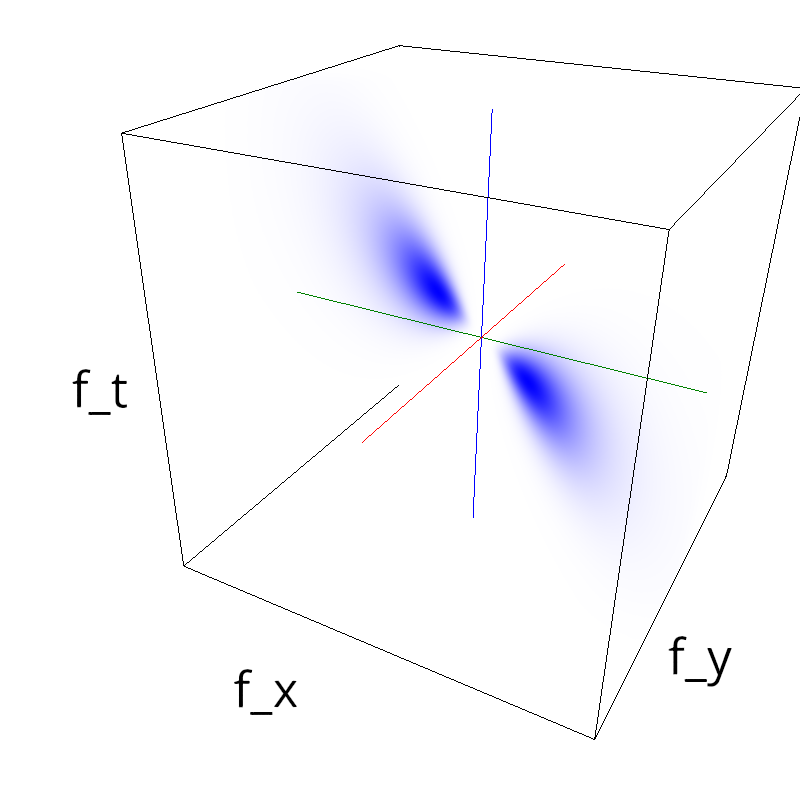
\includegraphics[width=.31\textwidth]{counterphase_grating.png}%
\\
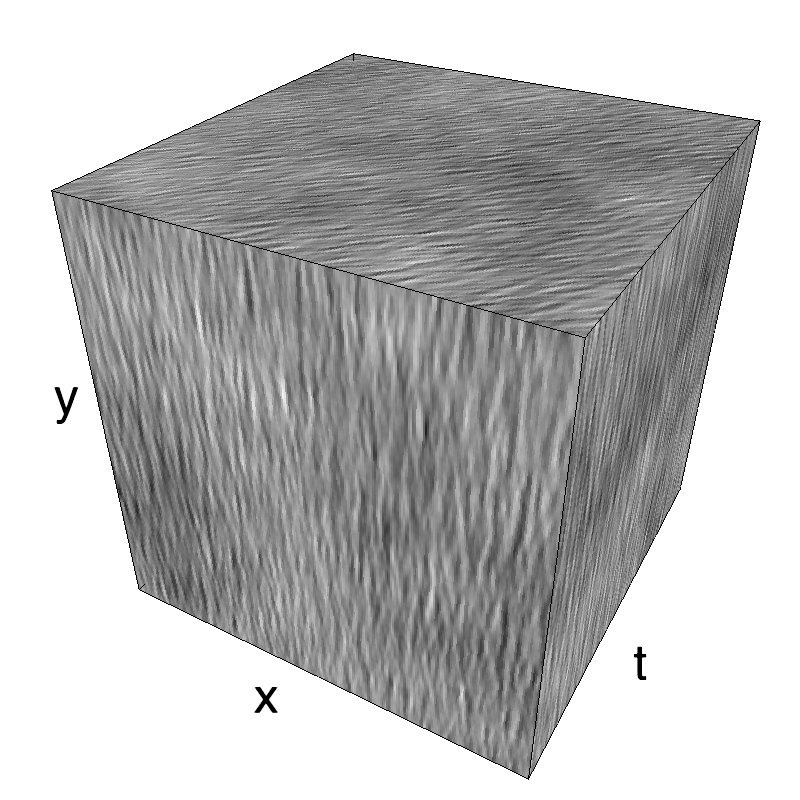
\includegraphics[width=.31\textwidth]{grating-noise_cube.png}&%
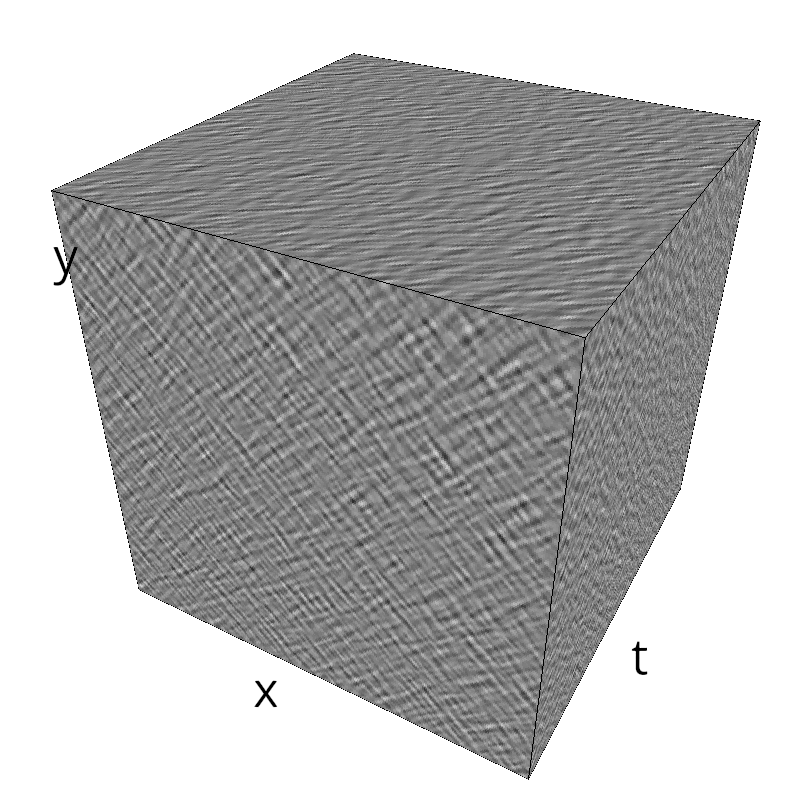
\includegraphics[width=.31\textwidth]{plaid_cube.png}&%
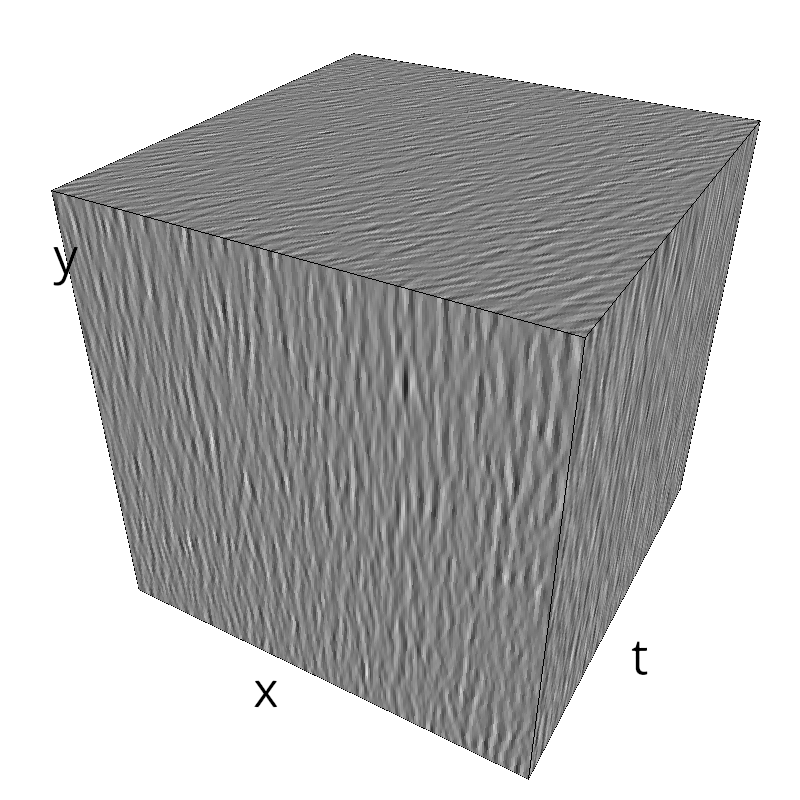
\includegraphics[width=.31\textwidth]{counterphase_grating_cube.png}%
\\%
\includemovie{.31\textwidth}{.31\textwidth}{results/grating-noise.mp4}&
\includemovie{.31\textwidth}{.31\textwidth}{results/plaid.mp4}&
\includemovie{.31\textwidth}{.31\textwidth}{results/counterphase_grating.mp4}%
\end{tabular}
\end{center}
	 \caption{Competing Motion Clouds. (\textit{A}): A narrow-orientation-bandwidth Motion Cloud with explicit noise. A red noise envelope was added to the global envelop of a Motion Cloud with a bandwidth in the orientation domain. (\textit{B}): Two Motion Clouds with same motion but different preferred orientation were added together, yielding a plaid-like Motion Cloud texture. (\textit{C}): Two Motion Clouds with opposite velocity directions were added, yielding a texture similar to a "counter-phase" grating. Note yet that the crossed shape in the $f_x-f_t$ plane is a signature of the opposite velocity directions, while two gratings with the same spatial frequency and in opposite directions would generate a flickering stimulus with energy concentrated on the $f_t$ plane.} %
	 \label{fig:counterphase} %
\end{figure} %

\end{document}%
